\documentclass[11pt]{amsart}

%\usepackage[notref,notcite]{showkeys}
\usepackage[style=nature, date=year]{biblatex}
\usepackage{float}
\usepackage{graphicx}
\usepackage{todonotes}
\usepackage{subcaption}
\usepackage{amsmath}
\usepackage{amsthm}
\usepackage{amssymb}
\usepackage{algorithm}
\usepackage[noend]{algorithmic}
\usepackage[foot]{amsaddr}
\usepackage[misc]{ifsym}
\usepackage{enumitem}
\usepackage{geometry}
\usepackage[hidelinks]{hyperref}

%FOCS&SODA margins
\setlist{leftmargin = 0pt, labelindent = 0pt}
\geometry{margin=1in}

\renewbibmacro{in:}{}
\addbibresource{rnni_polynomial.bib}
% Remove languages from bibliography
\AtEveryBibitem{
  \clearlist{language}
}

\newtheorem{proposition}{Proposition}
\newtheorem{theorem}{Theorem}
\newtheorem{lemma}{Lemma}
\newtheorem{corollary}{Corollary}
\newtheorem{problem}{Problem}
\newtheorem{conjecture}{Conjecture}

\newcommand{\rnni}{\mathrm{RNNI}}
\newcommand{\findpath}{\textsc{FindPath}}
\newcommand{\mrca}{\mathrm{mrca}}
\newcommand{\rank}{\mathrm{rank}}
\newcommand{\nni}{\mathrm{NNI}}
\newcommand{\spr}{\mathrm{SPR}}
\newcommand{\tbr}{\mathrm{TBR}}
\newcommand{\fp}{\mathrm{FP}}
\newcommand{\np}{\mathcal{NP}}
\newcommand{\p}{\mathcal{P}}
\newcommand{\decprob}[1]{\rnni(#1)\text{-}\mathrm{SP}}
\renewcommand{\O}{\mathcal O}
\renewcommand{\epsilon}{\varepsilon}

\newcommand{\sidma}[1]{\todo[color=green]{#1}}

% \newcommand{\summary}[1]{\textbf{#1}} % Print summaries to .pdf
\newcommand{\summary}[1]{} % Hide summaries in .pdf

\renewcommand{\thesubfigure}{\Alph{subfigure}}

\graphicspath{{figures/}}


\title[Computing $\rnni$ distance]{The complexity of computing nearest neighbour interchange distances between ranked phylogenetic trees}
\date{\today}
\author{Lena Collienne\textsuperscript{1}}
\email{lena.collienne@postgrad.otago.ac.nz}
\address{\textsuperscript{1}Department of Computer Science, University of Otago, New Zealand}
\author{Alex Gavryushkin\textsuperscript{1, \Letter}}
\email{\textsuperscript{\Letter}alex@biods.org}
\thanks{We acknowledge support from the Royal Society of New Zealand through a Rutherford Discovery Fellowship (RDF-UOO1702) awarded to AG.
This work was partially supported by Ministry of Business, Innovation, and Employment of New Zealand through an Endeavour Smart Ideas (CONT-61378-ENDSI-UOO) grant and a Data Science Programmes grant.}
\thanks{We thank Alexei Drummond and Kieran Elmes for useful discussions about the weight difference between $\rnni$ moves, scalability and applied aspects of our results, and the generalisation to discrete time-trees.
Their comments improved our paper.}



\begin{document}

\begin{abstract}
Many popular algorithms for searching the space of leaf-labelled (phylogenetic) trees are based on tree rearrangement operations.
Under any such operation, the problem is reduced to searching a graph where vertices are trees and (undirected) edges are given by pairs of trees connected by one rearrangement operation (sometimes called a move).
Most popular are the classical nearest neighbour interchange, subtree prune and regraft, and tree bisection and reconnection moves.
The shortest path problem, however, is $\np$-hard in each of these graphs, making tree inference and comparison algorithms challenging to design in practice.

Although ranked phylogenetic trees are one of the central objects of interest in applications, the computational complexity of the shortest path problem for these trees remained unsolved for decades.
In this paper, we settle this problem for the ranked nearest neighbour interchange operation by establishing that the complexity depends on the weight difference between two types of tree rearrangement operations (rank moves and edge moves) in this graph, and varies from quadratic to $\np$-hard.
In particular, our result provides the first example of a phylogenetic tree rearrangement operation for which shortest paths, and hence the distance, can be computed efficiently.
Specifically, our algorithm scales to trees with thousands of leaves.

We also propose a study of the parameter for weight difference between move types, that changes the complexity of the shortest path problem in our graph from quadratic to $\np$-hard.
In this paper we will provide an insight into this approach, motivated by ideas developed in the beyond worst-case analysis framework.
\end{abstract}


\maketitle
\thispagestyle{empty}

\newpage

\setcounter{page}{1}

\summary{Motivation: many popular tree search algorithms are based on NNI (e.g. this \url{https://academic.oup.com/mbe/article/28/10/2731/973375} tool has been cited 40K+ times, see also references there to PhyML, RaxML, etc. -- they all use NNI); other applications include tree comparison methods, tree inference methods (proposal distributions), summary statistics, etc.}
The problem of reconstructing evolutionary histories from sequence data is central for many tree inference methods used in computational biology.
The most common approaches infer trees from sequences via maximum likelihood \autocite{Stamatakis2006-xb, Guindon2010-lo}, MCMC \autocite{Ronquist2003-eq, Suchard2018-tw, Bouckaert2019-yr}, distance-, or parsimony-based approaches \autocite{Tamura2011-ky}.
All these methods rely of various tree rearrangement operations \autocite{Semple2003-nj}, the most popular of which are nearest neighbour interchange ($\nni$), subtree prune and regraft ($\spr$), and tree bisection and reconnection ($\tbr$).
Hence the tree inference problem can be formulated as a graph search, where vertices are trees and edges are given by the tree rearrangement operation of interest.

\summary{Motivation: However, all known graph-based tree rearrangement distances, including NNI, are NP-hard, and it took many years and paper to prove that; so approach such as practical FPT algorithms is an active area of research to overcome the computational (cite Whidden).}
Classical results in mathematical phylogenetics imply that computing rearrangement distances between trees, that is, the minimum number of tree rearrangements necessary to convert one tree into another, is $\np$-hard \autocite{Dasgupta2000-xa, Bordewich2005-nx, Hickey2008-wv, Allen2001-ky} for all three rearrangement operations $\nni$, $\spr$, and $\tbr$.
We will formally introduce all necessary definitions later in the paper.
Intuitively, the difference between the three operations is how much change can be done to a tree by a single operation, with $\nni$ being the most local type of rearrangement and $\tbr$ the most global one.
Remarkably, it took over 25 years and a number of published erroneous attempts, as discussed in detail by \textcite{Dasgupta2000-xa}, to prove that the shortest path problem is $\np$-hard in $\nni$ \autocite{Dasgupta2000-xa}.
Similarly, incorrect proofs for $\spr$ have been discussed in the literature \autocite{Hein1996-em, Allen2001-ky}, before \textcite{Bordewich2005-nx} proved the $\np$-hardness result for rooted trees and \textcite{Hickey2008-wv} utilised this proof to establish the result for unrooted trees.
To facilitate practical applications, fixed parameter tractable algorithms for computing the $\spr$ distance have been developed over the years \autocite{Whidden2010-bw, Bordewich2005-nx, Whidden2018-fw}.
Although important, these algorithms remain impractical for large distances and are only applied to trees with a moderate number of leaves or those with small distances.
It is still unknown whether the fixed parameter tractability result holds in $\nni$, which makes the shortest paths problem in this graph even more challenging \autocite{Gavryushkin2018-ol}.

\summary{Historically, the complexity question was following hand in hand with the cluster property -- more history plus biological relevance of the property.}
The idea utilised by \textcite{Dasgupta2000-xa} to prove that the shortest path problem in $\nni$ is $\np$-hard stems from a result that shortest paths in $\nni$ do not preserve clusters \autocite{Li1996-zw}, that is, two trees sharing a cluster does not imply that all trees along a shortest path have that cluster.
Not only this counter-intuitive property eventually led to the computational hardness result, the property made little sense biologically as trees clustering the same set of sequences into a subtree should be closer to each other than to a tree that does not have that subtree.
Indeed, a shared cluster means that both trees support the hypothesis that this cluster has evolved along a subtree.
It was believed that this so-called cluster property and the computational complexity of the shortest path problem were related \autocite{Li1996-zw}, so the two questions have historically been studied simultaneously \autocite{Dasgupta2000-xa}.
However, there is little evidence to justify this connection.
For example, the cluster property holds in $\spr$ even though the shortest path problem is $\np$-hard there.

\summary{Paper summary in light of motivation: We've discovered the first efficiently computable distance, given by a parameter range in known tree spaces, and want to understand the reason for the complexity jump -- cite ``Beyond worst-case complexity.''}
In this paper, we establish that for a certain tree rearrangement operation (a generalisation of $\nni$) the complexity of the shortest path problem is $\O(n^2)$ (Theorem~\ref{thm:rnni_polynomial}).
This is, to the best of our knowledge, the first tree rearrangement operation with polynomial-time computable shortest paths and distances between trees.
Our algorithm is practical as it allows to compute distances between trees with thousands of leaves, while in the closely related $\nni$ graph this number is well smaller \autocite{Li1996-zw, Whidden2016-kl} than 20.
To prove the main result of this paper, Theorem~\ref{thm:rnni_polynomial}, we will introduce the algorithm $\findpath$ and show that it computes shortest paths in the ranked nearest neighbour interchange graph ($\rnni$) in polynomial time.
We will also prove that the $\rnni$ graph has the cluster property, which is an important distinction between this graph and $\nni$.
We then generalise the $\findpath$ algorithm to trees with arbitrary integer-valued branch lengths and show that the shortest path problem for such trees is also polynomial-time.
We will finish the paper by investigating the question of whether there exists a threshold at which the complexity shifts from $\np$-hard to polynomial.
Specifically, we introduce an edge weight parameter $\rho$ in the $\rnni$ graph and consider a parametrised graph $\rnni(\rho)$.
We show that the shortest path problem is $\np$-hard in $\rnni(0)$ and quadratic in $\rnni(1)$, so the complexity changes with $\rho$.

We propose to characterise the values of $\rho \geq 0$ for which the complexity of computing distances in the parametrised graph is polynomial.
We will provide some insights into this characterisation problem at the end of this paper.
The problem is similar in spirit to the beyond worst-case analysis framework \autocite{Roughgarden2019-to}, because, just like in our result, a $\gamma$-perturbation stable instance of the maximum cut problem is known \autocite{Roughgarden2019-to} to be $\np$-hard for small values of $\gamma$ and polynomial for larger values of $\gamma$.
Since the problem of identifying the value of $\gamma$ where the complexity switches has largely been resolved \autocite{Makarychev2014-ev}, we hope that the approaches reviewed by \textcite{Roughgarden2019-to} will be helpful for this study.


\section{Definitions and background results}

\summary{Defining ranked trees and clusters.}
Unless stated otherwise, by a \emph{tree} in this paper we mean a \emph{ranked phylogenetic tree}, which is a binary tree where leaves are uniquely labelled by elements of the set $\{a_1, \ldots, a_n\}$ for a fixed integer $n$, and all internal (non-leaf) nodes are uniquely \emph{ranked} by elements of the set $\{1, \ldots, n-1\}$ so that each child has a strictly smaller rank than its parent.
All leaves are assumed to have rank $0$ but we only refer to the ranks of internal nodes throughout.
In total there are $\frac{(n - 1)! n!}{2^{n-1}}$ such trees on $n$ leaves \autocite{Gavryushkin2018-ol}.
Two trees are considered to be identical if there exists an isomorphism between them which preserves edges, leaf labels, and node rankings.
For example, trees in Figure~\ref{fig:ranked_trees_ex} are all different.

\begin{figure}[ht]
\centering
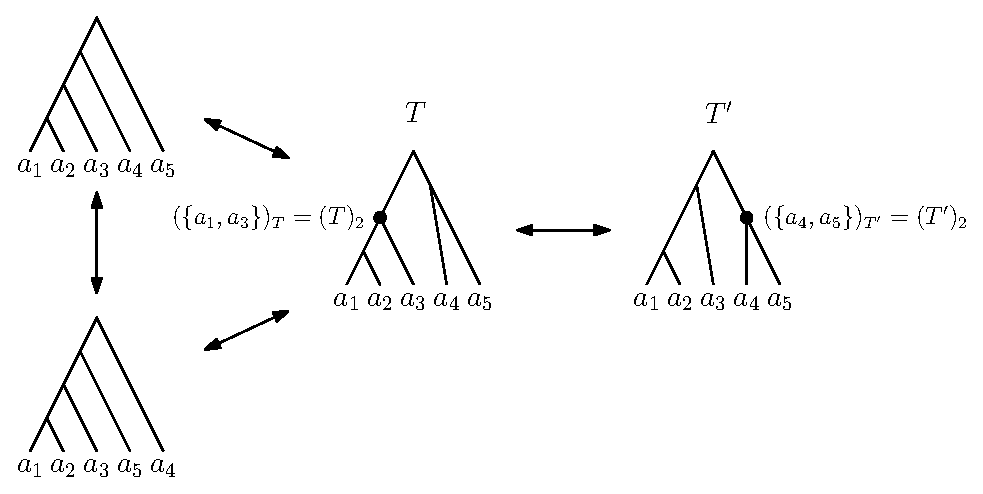
\includegraphics[width=0.8\textwidth]{ranked_trees_ex}
\caption{Trees in the $\rnni$ graph with three $\nni$ moves on the left and a rank move on the right.}
\label{fig:ranked_trees_ex}
\end{figure}

Because internal nodes of a tree $T$ are ranked uniquely, we can address \textbf{the} node of rank ${t \in \{1, \ldots, n - 1\}}$, and we write $(T)_t$ to denote this node.
An \emph{interval} $[(T)_t,(T)_{t+1}]$ is defined by two nodes of consecutive ranks.
A \emph{cluster} $C \subseteq \{a_1, \ldots, a_n\}$ in a tree $T$ is a subset of leaves that contains all leaves descending from one internal node of $T$.
We then say that this internal node \emph{induces} the cluster $C$, and that the subtree rooted at this node is \emph{induced} by $C$.
Trees can uniquely be specified using the \emph{cluster representation}, that is a list of all clusters induced by internal nodes of that tree ordered according to the ranks of internal nodes.
For example, the cluster representation of tree $T$ in Figure~\ref{fig:ranked_trees_ex} is $[\{a_1, a_2\}, \{a_1, a_2, a_3\}, \{a_4, a_5\}]$.
For a set $S \subseteq \{a_1, \ldots, a_n\}$ and tree $T$ we denote the \emph{most recent common ancestor} of $S$ in $T$, that is the node of the lowest rank in $T$ that induces a cluster containing all elements of $S$, by $(S)_T$.
Note that $(C)_T = (T)_t$ if the cluster $C$ is induced by the node of rank $t$ in $T$.

\summary{Defining graph $\rnni(\rho)$.}
We are now ready to introduce our main object of study, a class of graphs $\rnni(\rho)$ for $\rho \geq 0$.
The vertices of the $\rnni(\rho)$ graph are trees as defined above.
Two trees are connected by an edge if one results from the other by performing one of the following two tree rearrangement operations:\\
(i) A \emph{rank move} on a tree $T$ exchanges the ranks of two internal nodes $(T)_t$ and $(T)_{t+1}$ with consecutive ranks, provided the two nodes are not connected by an edge in the tree $T$.\\
(ii) Trees $T$ and $R$ are connected by an \emph{$\nni$ move} if there are edges $e$ in $T$ and $f$ in $R$ both connecting nodes of consecutive ranks in the corresponding trees, such that the trees resulting from shrinking $e$ and $f$ to internal nodes gives two identical (non-binary) trees.\\
Figure~\ref{fig:ranked_trees_ex} gives examples of these tree rearrangements.
The parameter $\rho \geq 0$ is the weight of the rank move operation, the $\nni$ moves weigh $1$.
The \emph{weight of a path} is the sum of the weights of all moves along the path.
The \emph{distance} between two trees in $\rnni(\rho)$ is the weight of a path with the minimal weight, which we will call a shortest path.
We first consider $\rho = 1$, so all edges in the graph have weight $1$ and we assume in this case that the graph is unweighted.

Our main object of study is the following class of shortest path problems parametrised by a non-negative real number $\rho$.

\medskip

\noindent $\decprob{\rho}$
\medskip\\
INSTANCE: A pair of trees $T$ and $R$\\
FIND: A path of minimal weight between $T$ and $R$ in $\rnni(\rho)$

\medskip

Our first goal is to prove that $\decprob{1}$ is polynomial-time solvable.
We will see later in the paper that it follows from a classical result \autocite{Dasgupta2000-xa} that $\decprob{0}$ is $\np$-hard.
We will also study $\decprob{\rho}$ for other values of $\rho$.
To be consistent with notations used in the literature \autocite{Gavryushkin2018-ol}, we will denote the graph $\rnni(1)$ by $\rnni$.


\section{Complexity of computing $\rnni$ distances}
\label{sec:rnni_complexity}

\summary{Introducing $\findpath$.}
In this section we will prove that the shortest path problem in $\rnni$ is polynomial-time solvable.
Our proof will be constructive -- we will show that the following quadratic algorithm, called $\findpath$, computes a shortest path between two given trees in $\rnni$.
$\findpath$ algorithm receives two trees $T$ and $R$ in their cluster representation.
We denote the representation of $R$ by $[C_1, \ldots, C_{n-2}]$.
The algorithm considers the clusters $C_1, \ldots, C_{n-2}$ iteratively in their order and produces a sequence $p$ of trees which becomes a shortest path from $T$ to $R$ after the algorithm terminates.
During each iteration $k = 1, \ldots, n-2$ new trees are added to $p$ if necessary, and we will refer to the last added tree as $T'$.
In iteration $k$, the rank of $(C_{k})_{T'}$ is decreased by $\rnni$ moves until $C_k$ is induced by the node of rank $k$ in $T'$.
Before proving that $\findpath$ computes shortest paths in $\rnni$, we show that $\findpath$ is a deterministic algorithm with running time quadratic in the number of leaves $n$.
In particular, there always exists a unique move that decreases the rank of $(C_{k})_{T'}$ as described above.

\begin{algorithm}[H]
\caption{$\findpath$($T,R$)}
\begin{algorithmic}[1]
\STATE $T' := T$, $p := [T']$, $[C_1, \ldots, C_{n-2}] := R$
\FOR {$k = 1, \dots, n-2$}
\label{alg:findpath:line:for_loop}
	\WHILE {$\rank((C_k)_{T'})>k$}
	\label{alg:findpath:line:while_loop}
		\IF {$(C_k)_{T'}$ and node $u$ with rank one less than $(C_k)_{T'}$ are connected by an edge}
			\STATE $T''$ is $T'$ with the rank of $(C_k)_{T'}$ decreased by an $\nni$ move
		\ELSE
			\STATE $T''$ is $T'$ with ranks of nodes $u$ and $(C_k)_{T'}$ swapped
		\ENDIF
		\STATE $T' = T''$
		\STATE $p = p+T'$
	\ENDWHILE
\ENDFOR
\RETURN $p$
\end{algorithmic}
\end{algorithm}

%%%%%%%%%% START from rnni_convexity paper
\begin{proposition}
$\findpath$ is a correct deterministic algorithm.
\end{proposition}

\proof
To show that the algorithm terminates with a path ending in $R$, we need to show that in the \textbf{for} loop (line~\ref{alg:findpath:line:for_loop}) there is always exactly one $\rnni$ move possible to decrease the rank of $(C_k)_{T'}$, until it is $k$.
Then it follows that the first $k$ clusters of $T'$ and $R$ coincide after iteration $k$ and hence after $n-2$ iterations the path has to arrive at $R$.

To complete the proof, it suffices to show that there is a unique $\rnni$ move that decreases the rank of $(C_k)_{T'}$, which proves that there is a unique, well-defined update operation in each execution of the \textbf{while} loop (line~\ref{alg:findpath:line:while_loop}).
For proving this, we consider the case $k = 1$ and $k>1$ separately.

Case $k = 1$.
In this case $C_k$ consists of two leaves $\{x, y\}$.
The node $v = (\{x, y\})_{T'}$ has rank $r > 1$.
Consider the node $w$ preceding $v$ in $T'$, that is, it has rank $r - 1$.
If a rank move that swaps $v$ and $w$ is possible then this is the only move on $T'$ that can decrease the rank of $(\{x, y\})_{T'}$.
If the rank move is impossible then there is an edge in $T'$ connecting $v$ and $w$.
The only way to decrease the rank of $(\{x, y\})_{T'}$ then is to perform an $\nni$ move on that edge.
It is not hard to see that out of two possible $\nni$ moves only one decreases the rank of this most recent common ancestor.

\sidma{Define the term "supress" in terms of ranked trees.}
Case $k > 1$.
\begin{enumerate}
\item $C_k = C_i \cup C_j$ for $i, j < k$.
Suppress $C_i$ and $C_j$ in both $T'$ and $R$ to new leaves $c_i$ and $c_j$ respectively and proceed as in Case $k = 1$.
\item $C_k = C_i \cup \{x\}$, where $x$ is a leaf not present in $C_1, \ldots, C_k$.
Suppress $C_i$ in both $T'$ and $R$ to a new leaf $c_i$ and proceed as in Case $k = 1$.
\item $C_k = \{x, y\}$ where both $x$ and $y$ are not in $C_1, \ldots, C_k$.
Proceed as in Case $k = 1$.
\sidma{The end of the proof is missing. Complete the proof. }
\end{enumerate}
\endproof

\sidma{While is highly likely that the worst-case complexity is quadratic, you need to demonstrate why that is the case. The simplest, and most convincing way would be to write this as a proposition and then go line-by-line detailing the running time.}
Clearly, the worst-case complexity of $\findpath$ is quadratic in the number of leaves.
%%%%%%%%%% END from rnni_convexity paper

\summary{A few words about the main theorem and its proof.}
The following theorem, that $\decprob{1}$ is polynomial, is the main result of our paper.
The proof of the theorem reduces the problem to establishing a local property (see~(\ref{eqn:iff_inequality}) below) about the $\findpath$ algorithm.
The property can intuitively be understood as $\findpath$ always choosing the best tree possible to go to.
Importantly, this result can be used for an arbitrary vertex proposal algorithm in an arbitrary graph to establish that the algorithm computes a shortest path between vertices in the graph, hence our proof technique is of general interest.

\begin{theorem}
The time complexity of the shortest path problem in the $\rnni$ graph on trees with $n$ leaves is $\O(n^2)$.
\label{thm:rnni_polynomial}
\end{theorem}

\proof
We prove this theorem by showing that for every pair of trees $T$ and $R$, the path computed by the $\findpath$ algorithm is a shortest $\rnni$ path.
We denote this path by $\fp(T, R)$ and its length by $|\fp(T, R)|$.

Assume to the contrary that $T$ and $R$ are two trees with a minimum distance $d(T, R)$ such that $d(T,R) \neq |\fp(T,R)|$, that is, $d(T,R) < |\fp(T,R)|$.
Let $T'$ be the first tree on a shortest $\rnni$ path from $T$ to $R$.
Then $d(T',R) = d(T, R) - 1$, implying that the distance between $T'$ and $R$ is strictly smaller than that between $T$ and $R$.
Hence $d(T', R) = |\fp(T',R)| < |\fp(T,R)| - 1$.
We finish the proof by showing that no trees satisfy this inequality.

Specifically, we will show that
\begin{equation}
\begin{split}
\mbox{for all trees $T$, $R$, and $T'$}	& \mbox{ such that $T'$ is one $\rnni$ move away from $T$,}\\
					&|\fp(T',R)| \geq |\fp(T,R)| - 1
\end{split}
 \label{eqn:iff_inequality}
\end{equation}

We will use Figure~\ref{fig:proof_idea} to demonstrate our argument.

\begin{figure}[ht]
\centering
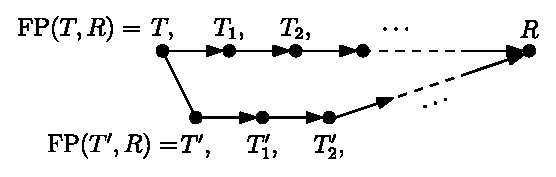
\includegraphics[width=0.6\textwidth]{proof_idea_ag}
\caption{Trees $T$, $T'$, and $R$ as in inequality~(\ref{eqn:iff_inequality}).
Paths $\fp(T,R) = [T,T_1,T_2, \ldots, R]$ and $\fp(T',R) = [T',T'_1,T'_2, \ldots, R]$ are indicated by arrows.}
\label{fig:proof_idea}
\end{figure}

Assume to the contrary that $T$ and $R$ are trees for which there exists $T'$ violating inequality~(\ref{eqn:iff_inequality}).
Out of all such pairs $T, R$ choose one with the minimal $|\fp(T, R)|$.
Denote $\fp(T,R) = [T, T_1, T_2, \ldots, R]$ and $\fp(T', R) = [T', T_1', T_2', \ldots, R]$, and let $[(T)_t, (T)_{t+1}]$ be the interval in $T$ on which the $\rnni$ move connecting $T$ and $T'$ is performed.
Let $C_k$ be the cluster of $R$ such that the node $(C_k)_T$ is moved down by the first move on $\fp(T, R)$.
If the rank of $(C_k)_T$ is not in $\{t, t+1\}$ then $(C_k)_T$ and $(C_k)_{T'}$ induce the same cluster, so $\findpath$ would make the same rearrangement in both trees $T$ and $T'$ in the first move along $\fp(T, R)$ and $\fp(T', R)$ resulting in trees $T_1$ and $T_1'$ which are $\rnni$ neighbours, as in Figure~\ref{fig:proof_idea}.
In this case, paths $\fp(T_1, R)$ and $\fp(T_1', R)$ violate inequality~(\ref{eqn:iff_inequality}) but $\fp(T_1, R)$ is strictly shorter than $\fp(T, R)$, contradicting our minimality assumption.
Hence, the first move on $\fp(T, R)$ has to involve an interval incident to at least one of the nodes $(T)_t$, $(T)_{t+1}$.

We will distinguish two cases depending on whether $T$ and $T'$ are connected by an $\nni$ or a rank move.
For each of these we will further distinguish all possible moves between $T$ and $T_1$.
Note that in all figures illustrating possible moves on $\fp(T,R)$ and $\fp(T',R)$, the positions of tree roots are irrelevant, so we have positioned roots to simplify our figures.

\textbf{Case 1.}
$T$ and $T'$ are connected by an $\nni$ move, so $((T)_t,(T)_{t+1})$ is an edge in $T$ -- see Figure~\ref{fig:thm_fp_nni1}.
Denote the clusters induced by the children of $(T)_t$ by $A$ and $B$ and the cluster induced by the child of $(T)_{t+1}$ that is not $(T)_t$ by $C$, and assume that the $\nni$ move between $T$ and $T'$ exchanges the subtrees induced by clusters $B$ and $C$.
Additionally, denote the cluster induced by the child of $(T)_{t+2}$ that is not $(T)_{t+1}$ by $D$ -- see Figure~\ref{fig:thm_fp_nni1}.

\begin{figure}[ht]
\centering
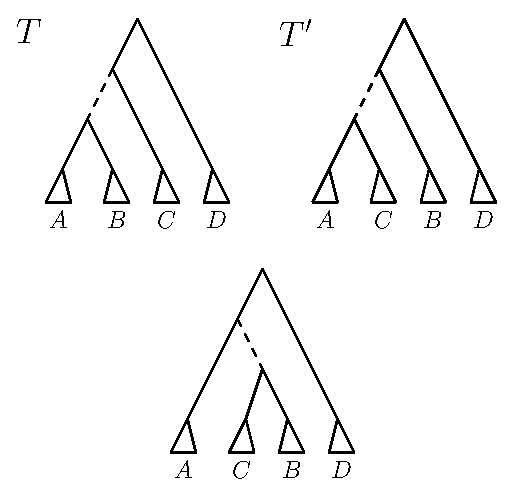
\includegraphics[width=0.35\textwidth]{thm_fp_nni1}
\caption{$\nni$ move between $T$ and $T'$ on the bold edge $((T)_t,(T)_{t+1})$ and the third $\rnni$ neighbour resulting from a move on that edge.}
\label{fig:thm_fp_nni1}
\end{figure}

We now consider all possible moves $\findpath$ can perform to go from $T$ to $T_1$ that involve a node of rank $t$ or $t+1$, that is, we will consider three intervals in total.

\begin{enumerate}[label = 1.{\arabic*}]
\item $\rnni$ move on interval $[(T)_t, (T)_{t+1}]$.
Note that this move has to be the $\nni$ move that is different from the $\nni$ move connecting $T$ and $T'$.

In this case, the cluster $B \cup C$ is built in $T_1$, as depicted in the bottom of Figure~\ref{fig:thm_fp_nni1}.
It follows that the cluster $C_k$ that is considered first by $\findpath$ must contain elements from both $B$ and $C$.
But then $\findpath$ applied to $T'$ and $R$ has to decrease the rank of $(C_k)_{T'}$ in its first step implying that $T'_1 = T_1$, so $|\fp(T',R)| = |\fp(T,R)|$.
This contradicts our assumption that $|\fp(T',R)| < |\fp(T,R)| - 1$.

\item $\nni$ move on (edge) interval $[(T)_{t+1}, (T)_{t+2}]$ that swaps the subtrees induced by clusters $C$ and $D$.
This move is shown in Figure~\ref{fig:thm_fp_nni2a} by an arrow from $T$ to the leftmost tree in the middle row.

\begin{figure}[ht]
	\begin{subfigure}[b]{.45\textwidth}
		\centering
		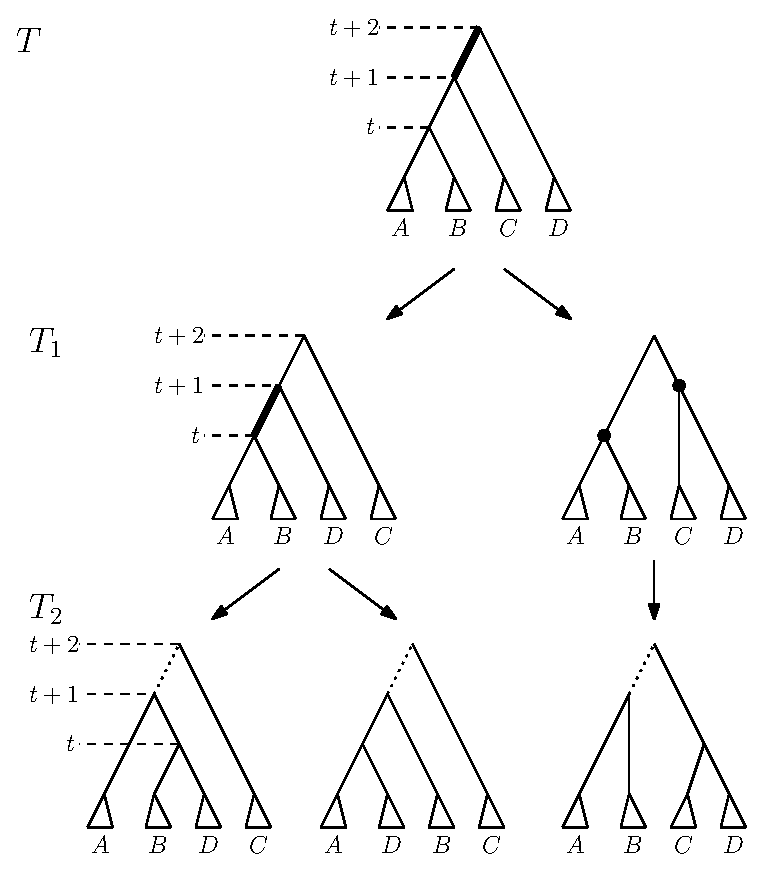
\includegraphics[width=0.9\linewidth]{thm_fp_nni2a.eps}
		\vspace{12pt}
		\caption{Possible initial segments of $\fp(T, R)$}
		\label{fig:thm_fp_nni2a}
	\end{subfigure}
	\begin{subfigure}[b]{.45\textwidth}
		\centering
		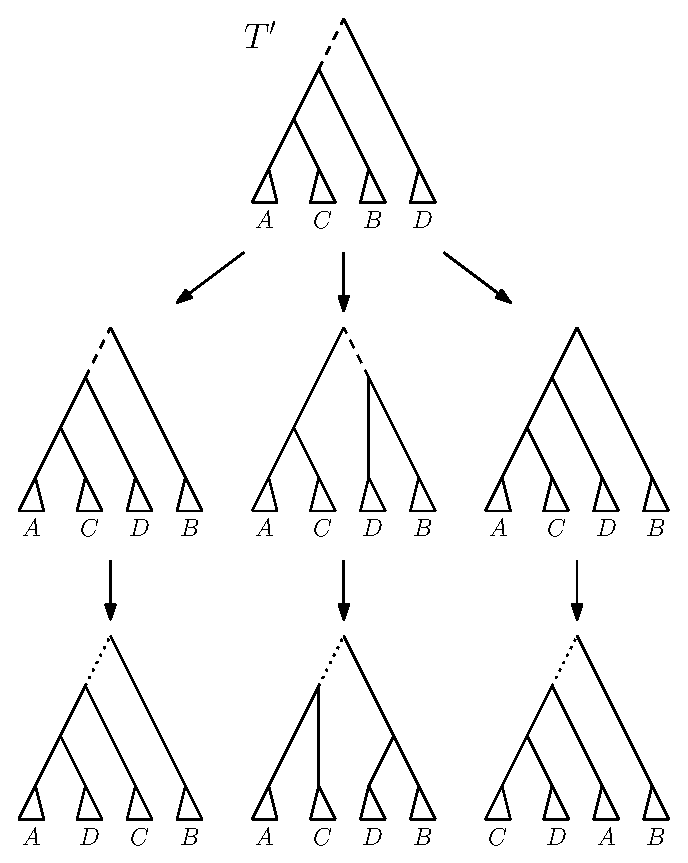
\includegraphics[width=0.9\linewidth]{thm_fp_nni2b.eps}
		\vspace{12pt}
		\caption{Possible initial segments of $\fp(T', R)$}
		\label{fig:thm_fp_nni2b}
	\end{subfigure}
	\caption{Comparison of paths $\fp(T, R)$ and $\fp(T', R)$ if $T$ and $T'$ are connected by an $\nni$ move on edge $((T)_{t+1},T_{t+2})$ in $T$.
	The bottom row displays all possibilities for $T_2$ and $T'_2$, depending on the position of cluster $C_k$ that is considered by $\findpath$:
	${C_k \subseteq B \cup D}$ is on the left, ${C_k \subseteq A \cup D}$ is in the middle, ${C_k \subseteq C \cup D}$ is on the right.}
	\label{fig:thm_fp_nni}
\end{figure}

Note that the cluster $C_k$ that is considered by $\findpath$ in the first step of computing $\fp(T, R)$ must intersect $D$.
Additionally, $C_k$ must intersect $A$, or $B$, or both of them.
Hence, we will consider each of these three cases individually.

We will use Figure~\ref{fig:thm_fp_nni} to demonstrate all three cases below.

\begin{enumerate}[label = \theenumi.\arabic*]
\item $C_k$ intersects each of $A$, $B$, and $D$.
We can assume $k > 1$ and $C_{k-1} = (R)_{k-1}$ as $C_1$ contains two elements and can therefore only intersect with either $A$ or $B$.
Since $C_k$ is the first cluster considered by $\findpath$, the two clusters that make up $C_k$ in $R$ must be present in $T$.
So $C_{k-1} = A \cup B$.
Since $A \cup B$ is not a cluster in $T'$, $\findpath$ will decrease the rank of $(C_{k-1})_{T'}$ on $\fp(T', R)$ before considering cluster $C_k$.
Note that the clusters induced by nodes of rank $i < k - 1$ in $T$ and $T'$ coincide, so all moves, if any, on $\fp(T, R)$ and $\fp(T', R)$ that involve those cluster will be the same.
The $\rnni$ move decreases the rank of $(C_{k-1})_{T'}$ by building the cluster $A \cup B$, in which case $T'_1 = T$.
This however contradicts $|\fp(T',R)| < |\fp(T,R)| - 1$.

\item $C_k \subseteq A \cup D$.
\label{deep_case_details}
Starting from $T$, $\findpath$ exchanges first subtrees induced by clusters $C$ and $D$ and then by $B$ and $D$.
This results in trees $T_1$ and $T_2$ -- see the path leading to the tree in the middle of the bottom row in Figure~\ref{fig:thm_fp_nni2a}.
Starting from $T'$, $\findpath$ exchanges first subtrees induced by $B$ and $D$ and then by $C$ and $D$.
This results in trees $T_1'$ and $T_2'$ -- see the path leading to the tree in the middle of the bottom row in Figure~\ref{fig:thm_fp_nni2b}.
It follows that $T_2$ and $T'_2$ only differ by one interval (indicated by dotted edges in the corresponding trees in Figure~\ref{fig:thm_fp_nni}), and hence are $\rnni$ neighbours.
This together with the facts that $|\fp(T_2,R)| = |\fp(T,R)|-2$ and $|\fp(T'_2,R)| = |\fp(T',R)|-2$ contradicts the assumption that $|\fp(T,R)|$ is a minimal length violating inequality~(\ref{eqn:iff_inequality}).

\item $C_k \subseteq B \cup D$.
This case is analogous to the previous one.
The two initial segments of $\fp(T, R)$ and $\fp(T', R)$ are the paths leading to the leftmost trees in the bottom row of Figures~\ref{fig:thm_fp_nni2a} and \ref{fig:thm_fp_nni2b}, respectively.
Note that the rank swap leading from $T_1'$ to $T_2'$ is required because the rank of $(C_k)_R$ is at most $t$ as implied by the move leading from $T_1$ to $T_2$.
The corresponding trees $T_2$ and $T_2'$ are again $\rnni$ neighbours.
\end{enumerate}

\item $\nni$ move on (edge) interval $[(T)_{t+1}, (T)_{t+2}]$ that builds a cluster $C \cup D$ in $T_1$.
\label{case:one_or_two_moves_down}
This move is shown in Figure~\ref{fig:thm_fp_nni2a} by an arrow from $T$ to the second leftmost tree in the middle row.
In this case, $C_k \subseteq C \cup D$.

If the ranks of $(C_k)_{T_1}$ and $(C_k)_R$ coincide then $C_{k-1} = A \cup B$ is a cluster in $R$.
Since $A \cup B$ is not a cluster in $T'$, the first $\rnni$ move on $\fp(T', R)$ builds the cluster $A \cup B$ by swapping subtrees induced by cluster $B$ and $C$.
This move results in $T_1' = T$ contradicting $|\fp(T',R)| < |\fp(T,R)| - 1$.

If the rank of $(C_k)_{T_1}$ is strictly higher than that of $(C_k)_R$ then $\findpath$ decreases the rank of $(C_k)_{T_1}$ in the second step.
This results in the path from $T$ to the rightmost tree in Figure~\ref{fig:thm_fp_nni2a}.
Hence, $\fp(T', R)$ also has to begin with two moves that decrease the rank of $(C_k)_{T'}$ twice, resulting in the rightmost path in Figure~\ref{fig:thm_fp_nni2b}.
Similarly to case~\ref{deep_case_details}, we arrive at a contradiction that trees $T_2$, $T_2'$, and $R$ violate inequality~(\ref{eqn:iff_inequality}) and $|\fp(T_2,R)| < |\fp(T,R)|$.

\item Rank move on interval $[(T)_{t+1},(T)_{t+2}]$.
\label{case:rank_move_interval_above}
This case is analogous to case~\ref{case:one_or_two_moves_down}.
If the ranks of $(C_k)_{T_1}$ and $(C_k)_R$ coincide then $C_{k-1} = A \cup B$ is a cluster in $R$, and applying $\findpath$ to $T', R$ we get $T'_1 = T$.
If the rank of $(C_k)_{T_1}$ is strictly higher than that of $(C_k)_R$ then $\findpath$ decreases the rank of $(C_k)_{T_1}$ in the second step.
Recall that the interval between nodes of rank $t$ and $t+1$ is an edge in both $T$ and $T'$.
Hence, the first two moves on $\fp(T', R)$ decrease the rank of $(C_k)_{T'}$ twice resulting in $T'_2$ which is an $\rnni$ neighbour of $T_2$ as depicted in Supplementary Figure~\ref{fig:thm_fp_nni3}.
As before, this contradicts our minimality assumption.

\item $\rnni$ move on interval $[(T)_{t-1},(T)_t]$.
In this case $C_k \subseteq A \cup B$, so the first move on $\fp(T', R)$ decreases the rank of $(C_k)_{T'}$ by exchanging the subtrees induced by $B$ and $C$.
This results in $T'_1 = T$.
This argument applies whether or not $((T)_{t-1},(T)_t)$ is an edge in $T$.
\end{enumerate}

\textbf{Case 2.}
$T$ and $T'$ are connected by a rank move on the interval between nodes of rank $t$ and $t+1$.
Denote the cluster induced by $(T)_t$ by $A$, the clusters induced by the children of $(T)_t$ by $A_1$ and $A_2$, the cluster induced by $(T)_{t+1}$ by $B$, and the clusters induced by the children of $(T)_{t+1}$ by $B_1$ and $B_2$ -- see Figure~\ref{fig:thm_fp_rank1}.

\begin{figure}[ht]
\centering
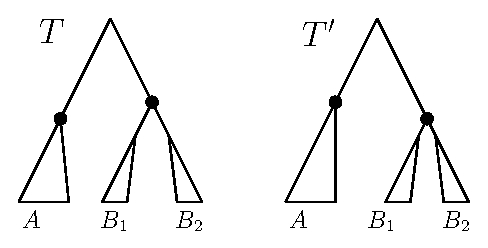
\includegraphics[width=0.4\textwidth]{thm_fp_rank1}
\caption{Rank move between $T$ and $T'$ on the interval above the node of rank $t$, and possible initial segments of $\fp(T, R)$ and $\fp(T', R)$.
We use notations ${A = A_1 \cup A_2}$ and $B = B_1 \cup B_2$.}
\label{fig:thm_fp_rank1}
\end{figure}

We again consider all possible moves $\findpath$ can perform to go from $T$ to $T_1$ that involve a node of rank $t$ or $t+1$.

\begin{enumerate}[label = 2.\arabic*]
\item Rank move on $[(T)_t,(T)_{t+1}]$.
This move results in $T_1 = T'$.

\item $\nni$ move on (edge) interval $[(T)_{t+1},(T)_{t+2}]$.
The following two sub-cases are analogous to case~\ref{case:one_or_two_moves_down}.

\begin{enumerate}[label = \theenumi.\arabic*]
	\item $(T)_{t+2}$ is a parent of $(T)_t$.
	The first move on $\fp(T, R)$ builds a cluster $A \cup B_1$ or $A \cup B_2$, and we assume without loss of generality that it is the former, as in Figure~\ref{fig:thm_fp_rank1}.
	This implies that $C_k \subseteq A \cup B_1$.
	If the ranks of $(C_k)_{T_1}$ and $(C_k)_R$ coincide then $C_{k-1} = A$ is a cluster in $R$.
	Therefore, the first move on $\fp(T', R)$ decreases the rank of $(A)_{T'}$, which results in $T_1' = T$.
	If the rank of $(C_k)_{T_1}$ is strictly higher than that of $(C_k)_R$ then $\findpath$ decreases the rank of $(C_k)_{T_1}$ in the second step.
	Due to the symmetry we can assume that $C_k \subseteq A_1 \cup B_1$, which implies that the move between $T_1$ and $T_2$ exchanges the subtrees induced by $A_2$ and $B_1$, as depicted on the left of Figure~\ref{fig:thm_fp_rank1}.
	$C_k \subseteq A_1 \cup B_1$ implies that the first two moves on $\fp(T', R)$ result in a tree $T'_2$ that is an $\rnni$ neighbour of $T_2$ -- see Figure~\ref{fig:thm_fp_rank1}.
	This is a contradiction to the minimality assumption on $|\fp(T,R)|$.

	\item $(T)_{t+2}$ is not a parent of $(T)_t$.
	In this case, there exists a cluster $C$ induced by the child of $(T)_{t+2}$ which is different from the one that induces $B$ -- see Figure~\ref{fig:thm_fp_rank2}.
\begin{figure}[ht]
	\centering
	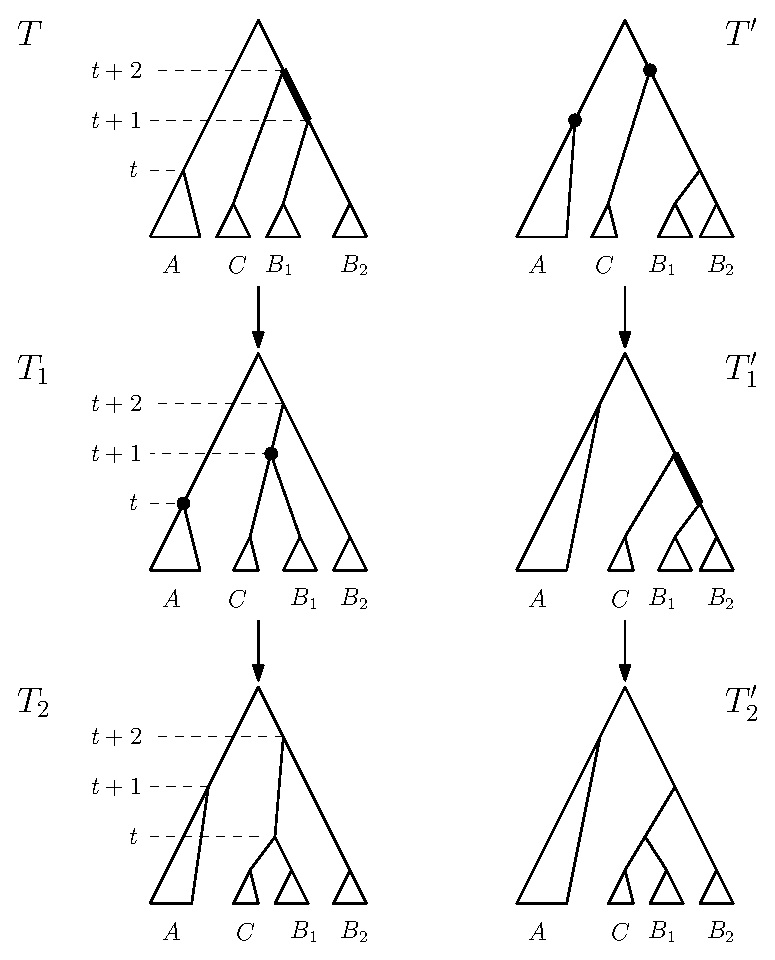
\includegraphics[width=0.4\textwidth]{thm_fp_rank2}
	\caption{Comparison of paths $\fp(T, R)$ and $\fp(T', R)$ if there is a rank move between $T$ and $T'$ and an $\nni$ move on the edge below the corresponding (rank) interval follows on $\fp(T, R)$.}
	\label{fig:thm_fp_rank2}
\end{figure}
	We can assume without loss of generality that $C_k \subseteq C \cup B_1$ and the first move on $\fp(T, R)$ builds a new cluster $C \cup B_1$.
	If the ranks of $(C_k)_{T_1}$ and $(C_k)_R$ coincide then $C_{k-1} = A$ is a cluster in $R$, which implies that $A$ is induced by the node of rank $t$ in both $T$ and $R$.
	So $T'_1 = T$.
	If the rank of $(C_k)_{T_1}$ is strictly higher than that of $(C_k)_R$ then $\findpath$ decreases the rank of $(C_k)_{T_1}$ in the second step -- see Figure~\ref{fig:thm_fp_rank2}.
	The corresponding first moves on $\fp(T', R)$ are shown on the right in Figure~\ref{fig:thm_fp_rank2}, and we again get that $T_2$ and $T_2'$ are $\rnni$ neighbours.
\end{enumerate}

\item Rank move on interval $[(T)_{t+1}, (T)_{t+2}]$.
Again, depending on whether or not the ranks of $(C_k)_{T_1}$ and $(C_k)_R$ coincide, we arrive at the conclusion that either $T_1' = T$ or $T_2$ and $T_2'$ are $\rnni$ neighbours, similar to case~\ref{case:rank_move_interval_above}.

\item $\rnni$ move on interval $[(T)_{t-1},(T)_t]$.
In this case $C_k \subseteq A$ and the first move on $\fp(T', R)$ must be a rank swap resulting in $T_1' = T$.
\end{enumerate}

Since all possible cases result in a contradiction, we conclude that inequality~(\ref{eqn:iff_inequality}) is true for all trees, which completes the proof of the theorem.
\endproof


\section{Applications}

In this section we apply Theorem~\ref{thm:rnni_polynomial} to settle further open problems about the $\rnni$ graph.

\subsection{Cluster Property}

\summary{Some words on the cluster property}
Historically in mathematical phylogenetics, the shortest path decision problem was studied hand in hand with the following cluster property \autocite{Dasgupta2000-xa}.
We say that a graph on trees has the \emph{cluster property} if for every pair of trees sharing a cluster it follows that every tree on every shortest path between the two trees also has this cluster.
Surprisingly, this property does not hold for the $\nni$ graph \autocite{Li1996-zw} and has been crucial for proving \autocite{Dasgupta2000-xa} that the shortest path problem in $\nni$ is $\np$-hard.
In this section, we will prove that the $\rnni$ graph has the cluster property by building on the fact that $\findpath$ computes shortest paths that preserve clusters.
Note that since paths computed by $\findpath$ preserve clusters, it follows directly that there always exists a shortest path that maintains every shared cluster.
However, the cluster property is universal and hence requires a proof that \textbf{all} shortest paths have this property.

\summary{Proving the Cluster Property for $\rnni$}

\begin{corollary}
Let $T$ and $R$ be two trees sharing a cluster $C$ and $p$ a shortest path from $T$ to $R$ in $\rnni$.
Then every tree on $p$ contains the cluster $C$.
\label{cluster_thm}
\end{corollary}

\proof
Assume to the contrary that $T$, $R$, $C$, and $p$ is a counterexample to the statement.
We can assume that no counterexample exists for paths shorter than $p$, so the first tree $T'$ after $T$ on $p$ does not contain the cluster $C$.
Therefore $T$ and $T'$ are connected by an $\nni$ move that moves a subtrees rooted at a child of $(C)_T$ out of the subtree induced by $C$ -- see Figure~\ref{fig:cluster_thm_proof}, where by $C_1$, $C_2$ we denote the clusters induced by the children of $(C)_T$.
Note that the only clusters in $T$ that distinguish $T$ from $T'$ are $C$ and the cluster induced by the node right above $(C)_{T}$, which is of the same rank as $(C)_{T'}$.

\begin{figure}[ht]
\centering
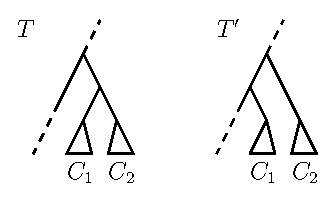
\includegraphics[width=0.3\textwidth]{cluster_thm_proof}
\caption{Neighbouring trees $T$ and $T'$, where $T$ contains the cluster $C = C_1 \cup C_2$ and $T'$ does not.
Dashed lines indicate identical parts of trees.}
\label{fig:cluster_thm_proof}
\end{figure}

Since $T$ and $R$ have the minimum distance among all counterexamples to the statement of the corollary, we can assume, using the same argument as in the beginning of proof of Theorem~\ref{thm:rnni_polynomial}, that $C$ is the first cluster considered by $\findpath$ on $\fp(T, R)$.
But in this case, the first move on $\fp(T',R)$ builds the cluster $C$ and results in tree $T$, which is a contradiction.
\endproof

\subsection{Generalisation to discrete time-trees}

\summary{Generalising $\findpath$ for discrete time-trees}
In this section we will show how to modify the $\findpath$ algorithm to efficiently solve the shortest path problem for \emph{discrete time-trees} \autocite{Gavryushkin2018-ol}.
These are trees where all internal nodes are uniquely ranked by elements of the set $\{1, \ldots, m\}$, where $m \geq n - 1$, so that children have strictly smaller ranks than their parents.
The NNI and rank moves are supplemented by a third type of move called a \emph{length move}, which changes (increases or decreases) the rank of an internal node by one without changing the rank of any other node in the tree.
So a length move implies that the length of one of the intervals $[(T)_{t+1},(T)_t]$ or $[(T)_t,(T)_{t-1}]$ for a $t \in \{2, \ldots, m-1\}$ increases by one and the other one decreases by one.
Note that $\nni$ moves are still only allowed on (edge) intervals bounded by consecutive nodes.

A natural extension of $\findpath$ to discrete time-trees is to simply add all the necessary length moves when a most recent common ancestor needs to be moved down to a particular level.
\begin{corollary}
The time complexity of the shortest path problem between discrete time-trees with $n$ leaves and node ranks bounded by $m$ is $\O(nm)$.
\label{cor:fp_dtt}
\end{corollary}

\proof
Let $T$ and $R$ be a pair of discrete time-trees.
We will convert $T$ and $R$ into $\rnni$ trees $T'$ and $R'$ on $m + 1$ leaves and show that the modified version of $\findpath$ for discrete time-trees is equivalent to the original $\findpath$ on converted trees.

To obtain $T'$, we add a new internal node of rank $m + 1$ as a new root.
We then add edges to attach this new root to the original root of $T$ and to the root of a new caterpillar tree with leaves labelled by $a_{n + 1}, \ldots, a_{m + 1}$.
The internal nodes of the caterpillar subtree in $T'$ are ranked by numbers for which there is no internal node of corresponding rank in the original tree $T$.
Note that all intervals of the resulting tree $T'$ are of length one.
We obtain $R'$ from $R$ in the same way using an identical caterpillar tree.

Now, a path $p$ between $T$ and $R$ can be transformed to a path $p'$ between $T'$ and $R'$ so that $|p| = |p'|$ by exchanging all length moves on $p$ to rank swaps on $p'$.
All rank moves and $\nni$ moves on $p'$ remain the same as on $p$.
In particular, this transformation matches the moves along $\fp(T,R)$ and $\fp(T',R')$ and Theorem~\ref{thm:rnni_polynomial} implies that $\fp(T, R)$ is a shortest path.
The running time bound follows from the running time of $\findpath$.
\endproof

Interestingly and in line with this result, the shortest path (geodesic) problem is polynomial-time computable in the continuous space of time-trees \autocite{Gavryushkin2016-uu}, where intervals can be of arbitrary real-valued lengths.
Note also that Corollaries~\ref{cluster_thm} and \ref{cor:fp_dtt} imply that the space of discrete time-trees has the cluster property.


\section{For what $\rho$ is $\decprob{\rho}$ polynomial?}

\summary{Summarising results on complexity of $\decprob{\rho}$ -- $\decprob{1} \in \p$ and $\decprob{0} \in \np$}
As we have seen in Section~\ref{sec:rnni_complexity}, the shortest path problem $\decprob{1}$ is solvable in polynomial time.
In this section, we will show that a classical result in mathematical phylogenetics implies that $\decprob{0}$ is $\np$-hard.
We will also discuss $\decprob{\rho}$ for other values of $\rho$.

\begin{theorem}[\textcite{Dasgupta2000-xa}]
$\decprob{0}$ is $\np$-hard.
\label{thm:nni_hard}
\end{theorem}

\proof
Note that the length of the path required in an instance of $\decprob{0}$ is equal to the minimum number of $\nni$ moves necessary to convert one tree into another tree where the rankings of internal nodes are ignored and every $\nni$ move is allowed on every edge.
This minimum is called the $\nni$ distance and the corresponding decision problem is known to be $\np$-hard \autocite{Dasgupta2000-xa}.
\endproof

\summary{Complexity of $\decprob{\rho}$ changes somewhere between zero and one -- where remains an open question}
In the light of Theorem~\ref{thm:rnni_polynomial} and Theorem~\ref{thm:nni_hard} the following problem is natural.

\begin{problem}
Characterise the complexity of $\decprob{\rho}$ in terms of $\rho$.
\label{prblm:rho_range}
\end{problem}

\summary{Getting one step closer to answer this question by considering small neighbourhoods for $\rho$ around zero and one}
We now show that Theorem~\ref{thm:nni_hard} can be extended to some values of $\rho$ close to $0$.
This suggests a possibility of a threshold $\hat\rho \in [0, 1]$ that separates the values of $\rho$ for which $\decprob{\rho}$ is polynomial from those for which $\decprob{\rho}$ is $\np$-hard.
Assuming the threshold exists, the following conjecture implies that $\hat\rho > 0$.

\begin{conjecture}
There exists $\delta > 0$ such that the shortest path problem $\decprob{\epsilon}$ is $\np$-hard for all $\epsilon < \delta$.
\label{prop:complexity_around_nni}
\end{conjecture}

%%%%%%%%%%%%%% START stuff from rnni_rho.tex
\summary{Finding one $\rho$ between $0$ and $1$ for which $\decprob{\rho} \notin \p$}
In the following we aim to find values for $\rho$ close to zero for which $\decprob{\rho}$ is not polynomial.

\begin{lemma}
    If $\decprob{\rho} \in \p$ for all $\rho > 0$, then it is $\rnni(0) \in \p$.
    \label{lemma:if_decprob_poly}
\end{lemma}

\proof
	Let $T$ and $R$ be trees and let $n$ be the number of their leaves.
    By the assumption of the lemma, shortest paths between these trees can be computed in any space $\rnni(\rho)$ for $\rho > 0$ in polynmoial time.
	Let $p_\epsilon$ be such a shortest path in $\rnni(\epsilon)$ with $\epsilon := \frac{1}{r+1}$
	\todo{$\epsilon$ or $\rho_0$? -- $\rho_0$ results in awkward indexing: $p_{\rho_0}$}
	, where $r = \Delta(\rnni)$ is the diameter
	\todo{do we need to prove the diameter here?}
	of $\rnni$.
    We will now show that the path $p_0$ in $\rnni(0)$ consisting of the same trees as $p_\epsilon$ is a shortest path in $\rnni(0)$.

    For contradiction we assume that there is a path $q_0$ shorter than $p_0$ in $\rnni(0)$.
    It follows $|q_0| \leq |p_0| - 1$.
    For the path $q_\epsilon$ in $\rnni(\epsilon)$ it is $|q_\epsilon| = |q_0| + m_r \epsilon < |q_0| + 1 \leq |p_0| \leq |p_\epsilon|$, where $m_r$ is the number of rank moves on $q_0$.
    Note that there cannot be more than $r$ rank moves $m_r$ on $q_0$ as we assumed that $q_0$ is a shortest path in $\rnni(0)$.
    However, $|q_\epsilon| < |p_\epsilon|$ contradicts the fact that $p_\epsilon$ is a shortest path in $\rnni(\epsilon)$.
\endproof

The following corollary is a direct result of Lemma~\ref{lemma:if_decprob_poly} and Theorem~\ref{thm:nni_hard}.

\begin{corollary}
    There is a $\rho_0 > 0$ for which $\decprob{\rho} \notin \p$.
    \label{cor:exists_rho_not_poly}
\end{corollary}

\summary{Finding a sequence of $\rho$s converging to zero for which the problem is not in $\p$.}

The following lemma is one step forward from Lemma~\ref{lemma:if_decprob_poly} towards constructing a sequence of values of $\rho$ for which $\decprob{\rho}$ is not polynmoial.

\begin{lemma}
    Let $0 < \rho_0 < 1$.
    If $\decprob{\rho} \in \p$ for all $0<\rho<\rho_0$, then it is ${\decprob{0} \in \p}$.
\end{lemma}

\proof
	This proof is analogous to the one of Lemma~\ref{lemma:if_decprob_poly}.
	To ensure $\epsilon < \rho_0$, pick $\epsilon := \min\{\frac{1}{r + 1}, \rho_0\}$.
\endproof

With the previous lemma and $\decprob{0} \notin \p$ (Theorem~\ref{thm:nni_hard}) we get the following result.

\begin{proposition}
    If $\decprob{\rho_0} \notin \p$, then exists a $\rho_1$ with $0 < \rho_1 < \rho_0$ such that ${\decprob{\rho_1} \notin \p}$.
    \label{proposition:more_rho_not_poly}
\end{proposition}

\begin{theorem}
    There is a sequence $\rho_0, \rho_1, \rho_2, \ldots$ with $1 > \rho_0 > \rho_1 > \rho_2 > \ldots > 0$ such that $\decprob{\rho_m} \notin \p$ for all $m \in \mathbb N$ and $\rho_m \underset{m \rightarrow \infty}{\longrightarrow} 0$.
\end{theorem}

\proof
    The Theorem follows from Corollary~\ref{cor:exists_rho_not_poly} and iteratively applying Proposition~\ref{proposition:more_rho_not_poly}.
\endproof
%%%%%%%%%%%%%% END stuff from rnni_rho.tex

Although the complexity of $\decprob{\rho}$ is not known for $\rho > 1$, the following proposition shows that the $\findpath$ algorithm is not applicable in this case.

\begin{proposition}
$\findpath$ does not compute shortest paths in $\rnni(\rho)$ for $\rho > 1$.
\label{prop:complexity_above_rnni}
\end{proposition}

\proof
The trees $[\{a_1,a_2\},\{a_1,a_2,a_3\},\{a_1,a_2,a_3,a_4\}]$ and $[\{a_3,a_4\},\{a_2,a_3,a_4\},\{a_1,a_2,a_3,a_4\}]$ give the required counterexample.
\endproof


\section{Open problems}

In this framework, we propose to study the following questions.
\begin{enumerate}
\item Problem~\ref{prblm:rho_range} above.
Additionally, as discussed in the introduction, since the cluster property is of importance in biological applications, the $\np$-hardness result can be interpreted as $\decprob{\rho}$ being hard only when the graph $\rnni(\rho)$ is biologically irrelevant.
We hence propose the following question.
For which values of $\rho$ does $\rnni(\rho)$ have the cluster property?


\item The questions we have considered for ranked $\nni$ can be studied in other rearrangement-based graphs on leaf-labelled trees, such as the ranked $\spr$ graph and the ranked $\tbr$ graph \autocite{Semple2003-nj}.
What is the complexity of the shortest path problem there?
Does the complexity depend on edge weights?

\item Can our results, e.g.\ the algorithm for computing shortest paths in $\rnni$, be used to establish whether the problem of computing geodesics between trees with real-valued time intervals is polynomial-time solvable?
This geodesic metric space is called $\mathrm t$-space and an efficient algorithm for computing geodesics in $\mathrm t$-space would be of importance for applications \autocite{Gavryushkin2016-uu}.
\end{enumerate}


\section*{Appendix}
\renewcommand{\figurename}{Supplementary Figure}

\begin{proof}[Detailed proof of Proposition~\ref{prop:complexity_above_rnni}]
We prove this proposition by a counterexample given by the trees \break $T = [\{a_1,a_2\},\{a_1,a_2,a_3\},\{a_1,a_2,a_3,a_4\}]$ and $R = [\{a_3,a_4\},\{a_2,a_3,a_4\},\{a_1,a_2,a_3,a_4\}]$.
For these trees $\findpath$ computes a path with the two trees trees $[\{a_1,a_2\},\{a_3,a_4\},\{a_1,a_2,a_3,a_4\}]$ and \break $[\{a_3,a_4\},\{a_1,a_2\},\{a_1,a_2,a_3,a_4\}]$ between $T$ and $R$.
This path consists of two $\nni$ moves with one rank move in between and therefore has weight $2 + \rho$.
However, there is a path from $T$ to $R$ with trees $[\{a_2,a_3\},\{a_1,a_2,a_3\},\{a_1,a_2,a_3,a_4\}]$ and $[\{a_2,a_3\},\{a_2,a_3,a_4\},\{a_1,a_2,a_3,a_4\}]$ between $T$ and $R$, which only consists of $\nni$ moves.
This path has weight $3$ and is therefore shorter than $\fp(T,R)$ for $\rho > 1$.
\end{proof}

The following figure illustrates Case~\ref{case:rank_move_interval_above} from the proof of Theorem~\ref{thm:rnni_polynomial}.

\begin{figure}[ht]
	\centering
	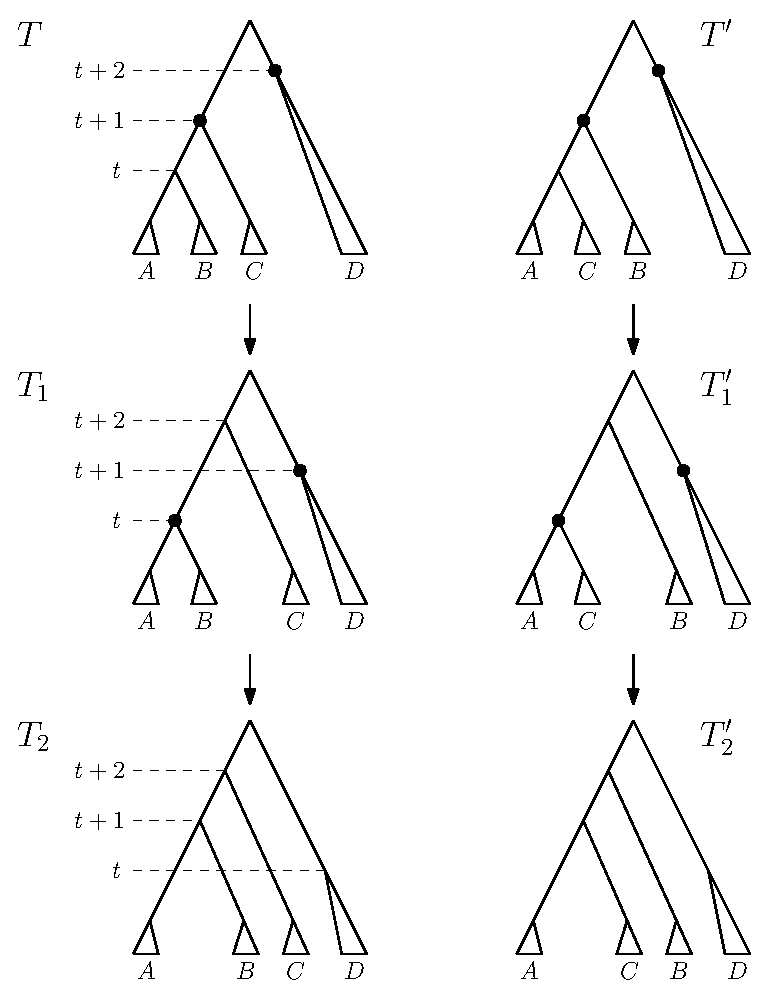
\includegraphics[width=0.4\textwidth]{thm_fp_nni3}
	\caption{Comparison of paths $\fp(T, R)$ and $\fp(T', R)$ if there is an $\nni$ move between $T$ and $T'$ and a rank move on the interval above this edge follows on $\fp(T, R)$.}
	\label{fig:thm_fp_nni3}
\end{figure}

\newpage
\printbibliography
\end{document}
